\section{CyPhyHouse Architecture}
\label{sec:middleware}
% \subsection{Approach}
\newcommand{\Shapeform}{\textit{Shapeform}\xspace}

A system running a Koord application has three parts: an application program, a controller, and a plant.
At runtime, the Koord program executes within the runtime system of a single agent, or a collection of programs execute on different agents that communicate using shared variables.
The plant consists of the hardware platforms of the participating agents.
The controller receives inputs from the program (through actuator ports), sends outputs back to the program (through sensor ports), and interfaces with the plant.
\iffalse
 \begin{wrapfigure}{r}{0.28\textwidth}
    \begin{center}
     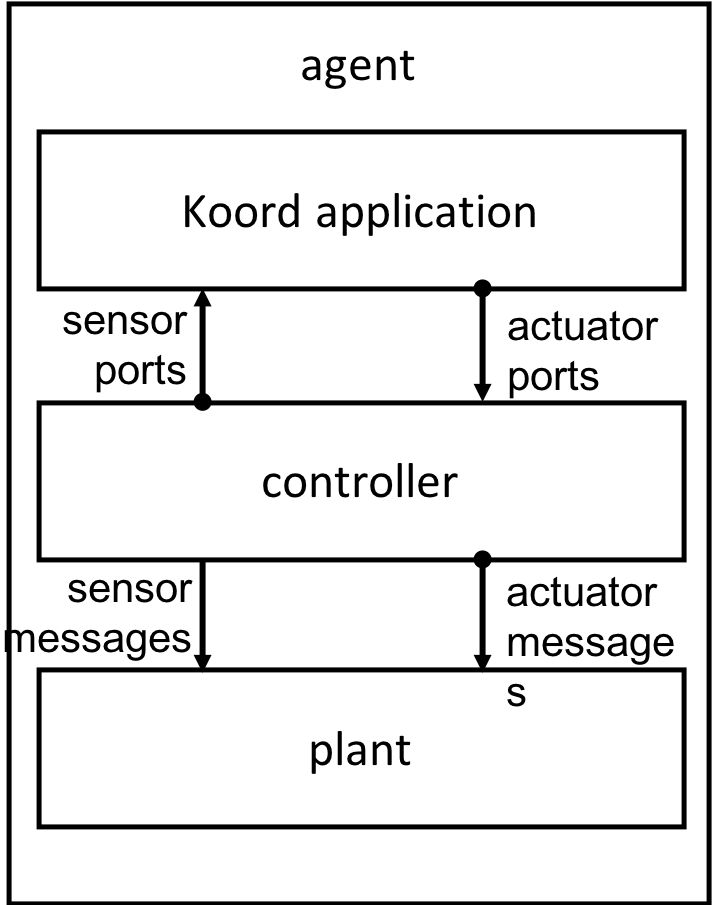
\includegraphics[width=0.28\textwidth,trim={0.3cm 0 0.3cm 0},clip]{figs/arch.png}
    \end{center}
    \caption{\small Three-plane architecture for a single agent: $\lgname$ program interfaces with its environment (controller and plant) through sensor and actuator ports.}
    \label{fig:arch}
\end{wrapfigure}
\fi

\subsection{Compilation}

The \rg{Koord compiler included with CyPhyHouse} generates Python code for the application using all the supported libraries,
such as the implementation of distributed shared variables using message passing over WiFi, motion automata of the robots, high-level collision and obstacle avoidance strategies, etc.
The application then runs with the Python \emph{middleware} for CyPhyHouse.
The Koord compiler is written using Antlr (Antlr 4.7.2) in Java~\cite{Parr:2013:DAR:2501720}.%
  ROS is used to handle the low-level interfaces with hardware.
To communicate between the high-level programs and low-level controllers, the middleware uses Rospy, a Python client library for ROS which enables the (Python) middleware to interface with ROS Topics and Services used for deployment or simulation.


\subsection{Shared memory and Communication}

At a high level, updates to a shared variable by one agent are propagated by the CyPhyHouse middleware, and become visible to other agents in the next round. The correctness of a program relies on agents having consistent values of shared variables. When an agent updates a shared variable, the middleware uses message passing to inform the other agents of the change. These changes should occur before the next round of computations.

CyPhyHouse supports UDP based messaging over Wi-Fi for communication between robots to implement the shared memory. Any shared memory update translates to a update message which the agent broadcasts over WiFi. The agents running a single distributed Koord application are assumed to be running on a single network node, with little to no packet loss. However, the communication component of the middleware can be easily extended to support multi-hop networks as well.
\begin{figure*}[!htbp]
\centering
 \begin{minipage}[b]{\textwidth}
    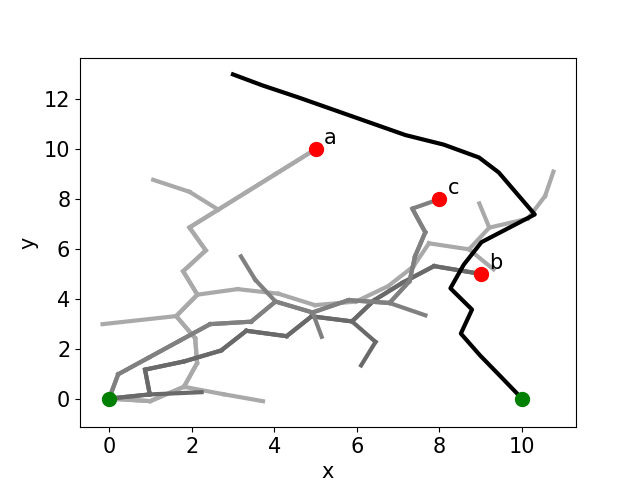
\includegraphics[width=0.33\textwidth]{figs/nonconflict.png}
    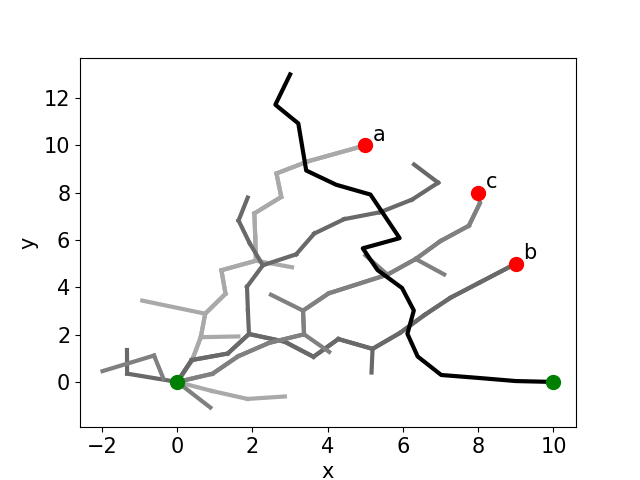
\includegraphics[width=0.33\textwidth]{figs/conflict.png}
    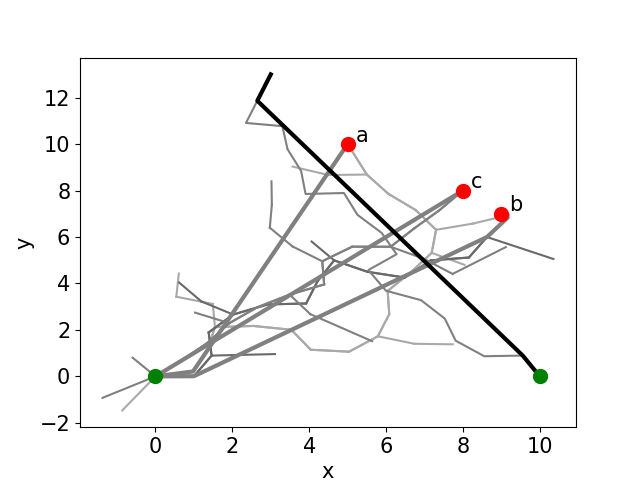
\includegraphics[width=0.33\textwidth]{figs/rrt_with_smoothing.png}
     \caption{\small Different planner can work with the same code. \emph{Left} shows the $x\-y$ plots of concurrently available paths  during a round of the \Task application using an RRT planner for two quadcopters. \emph{Middle} shows the same configuration, where paths computed are not viable to be traversed concurrently. The green markers are current quadcopter positions, The black path is a fixed path, and the red points are unsassigned task locations. \emph{Right} shows the same scenarios under which paths cannot be traversed concurrently, except that a different RRT-based planner (with path smoothing) is used.\vspace{-2mm}}
    \label{fig:pathplanners}
  \end{minipage}
\end{figure*}



\subsection{Dynamics}
If an application requires the agents to move, each agent uses an abstract class, \emph{Motion automaton}, which must be implemented for each hardware model (either in deployment or simulation).
This automaton subscribes to the required ROS Topics for positioning information of an agent, updates the \emph{reached} flag of the motion module, and publishes to ROS topics for motion-related commands, such as waypoint or path following. It also provides the user the ability to use different path planning modules as long as they support the interface functions. \reffig{pathplanners} shows two agents executing the \emph{same application} using different path planners.\vspace{-1mm}

\subsection{Portability}

Apart from the dynamics, all aforementioned components of the CyPhyHouse middleware are platform-agnostic.
My implementation allows any agent or system simulating or deploying a Koord program to use a configuration file to specify the system configuration, and the runtime modules for each agent, including the dynamics-related modules, while using the same application code.

\section{Deployment Setup}
\label{sec:hardware}
\subsection{Vehicles}

As previously mentioned, the CyPhyHouse\ toolchain was developed with heterogeneous robotics platforms in mind.
In order to demonstrate such capabilities, we have built both a car and a quadcopter.



\subsubsection*{Quadcopter}

The quadcopter was assembled from off-the-shelf hardware, with a $40 \text{cm} \times 40 \text{cm}$ footprint.
The main computing unit consists of a Raspberry Pi 3 B+ along with a Navio2 deck for sensing and motor control. 
Stabilization and reference tracking are handled by Ardupilot~\cite{ardupilot}.
Between the CyPhyHouse\ middleware and Ardupilot we include a hardware abstraction layer to convert setpoint messages from the high-level language into MAVLINK using the mavROS library (\cite{mavros}), so Ardupilot can parse them.
Since the autopilot was originally meant to use a GPS module, we also convert the current quadcopter position into the Geographic Coordinate System before sending it to the controller.


\subsubsection*{Car}

Similar to the quadcopter, the car platform uses off-the-shelf hardware based on the open-source MIT RACECAR project~\cite{MIT_RACECAR}.
The computing unit consists of an NVIDIA TX2 board.
In the car platform, instead of using Ardupilot to handle the waypoint following, we wrote a custom ROS node uses the current position and desired waypoints to compute the input speed and steering angle using a Model Predictive Controller (MPC).
The car has an electronic speed controller that handles low-level hardware control.
\begin{figure}[ht] 
%  \begin{minipage}[b]{0.5\linewidth}
%    \centering
    %\includegraphics[width=0.5\textwidth]{figs/time-vs-x.pdf}
%  \end{minipage}%%
%  \\
%  \begin{minipage}[b]{0.6\linewidth}
%    \centering
    %\includegraphics[width=0.5\textwidth]{figs/time-vs-y.pdf}
%  \end{minipage}
 \centering
  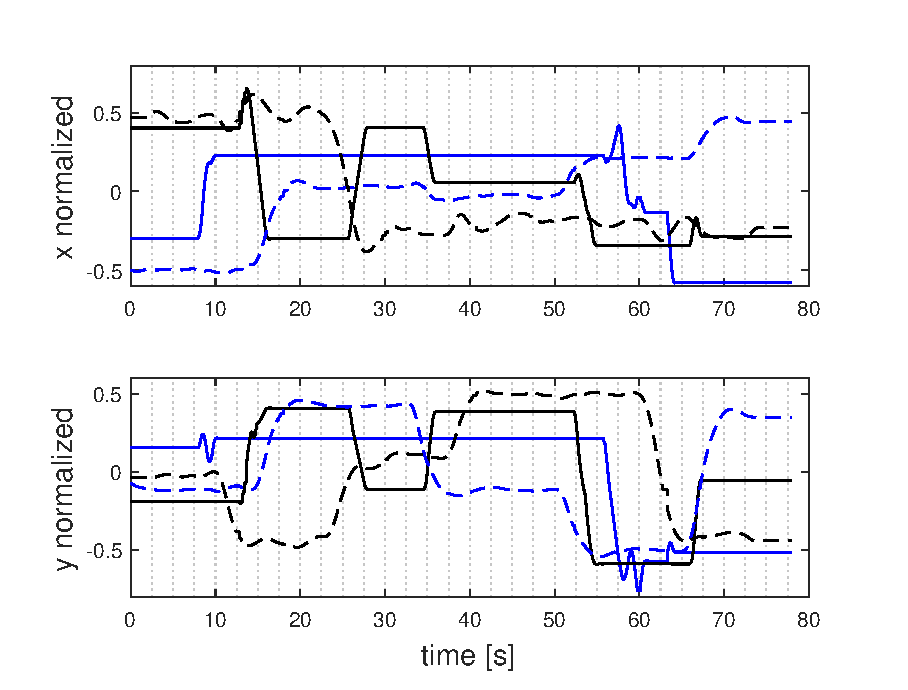
\includegraphics[scale=0.5]{figs/xyvst_norm.eps}
  
  \caption{\small \emph{Top} shows the $x\ vs\ t$ trajectories of the vehicles during an execution of the task, and \emph{bottom} shows the $y\ vs\ t$ trajectories. The vehicle positions were normalized to improve visualization. We can see concurrent movement when it is safe (for example at 13, 36, and 52 seconds), and only one robot moving or no robot moving when trying to compute a safe and collision-free path to a task.  }
  \label{fig:taskdepl}
  \end{figure}
\paragraph*{Test arena and localization}
The hardware experiments were performed in a $7 \text{m} \times 8 \text{m} \times 3 \text{m}$ arena equipped with 8 Vicon cameras.
The Vicon system allows us to track the position of multiple robots with sub-millimeter accuracy, however, the position data can come from any source (for example GPS, ultrawide-band, LIDAR), as long as all robots share the same coordinate system.
%
% Sayan: this is not important.
%The reflective markers used by the motion capture system can be seen in both vehicles in the inset figure in \reffig{realvis} (\emph{Right}).
%
While the motion capture system transmits all the data from a central computer, each vehicle only subscribes to its own position information.
%, discarding any extra data.
This was done to simplify experiments, as the goal of the paper is not to present new positioning systems.
%
All coordination and de-conflicting across agents is performed based on position information shared explicitly through shared variables in the Koord application.

\paragraph*{Interface with middleware}

As mentioned earlier in \refsect{middleware}, the same application can be deployed using different path planners, which are associated with the platform-specific \emph{motion automaton} through interfaces defined by the CyPhyHouse\ middleware. Both vehicles use RRT-based path planners~\cite{lavalle1998rapidly} to compute a path to the next task. For the car the RRT uses a bicycle model to compute the feasible paths, while for the quadcopter the RRT assumes it can move in a straight line between points.
%\fTBD{\sayan{shouldn't this be in the middleware section? around figure 5. OK to repeat and remind with reference back to middleware section.}}
%
The path generated is then forwarded to the robot via a ROS topic.
The ROS topics required for positioning and setting waypoints of the vehicles were specified in the configuration.
Each vehicle updates the \emph{reached} topic when they reach a predefined ball around the destination. 
Note that the car has nonholonomic constraints, while the quadcopter has uncertain dynamics, so in other standard settings, a roboticist would have to develop a separate application for each platform. 

\subsection{Experiments with \Task on upto four vehicles}
The \Task application of \refsect{overview} was run in over 100 experiments with different combinations of cars and quadcopters.
\reffig{taskdepl} shows the $(x,y)$-trajectories of the vehicles in one specific trial run, in which two  quadcopters and two cars were deployed. 
Careful examination of the figure  shows that all the performance requirements of \Task are achieved, with concurrent movement when different robots have clear paths to tasks, safe separation at all times, and agents getting blocked when there is no safe path found. In experiments with up to $4$ vehicles, with fewer agents, there were fewer blocked paths, so each robot spends less time idling, but this non-blocking effect is superseded by the parallelism gains obtained from  having multiple robots. For example, with three agents (2 quadcopters and 1 car, or 1 quadcopter and 2 cars) showing an average runtime of about 110 seconds for 20 tasks.
  The average runtime for the same with 4 agents across 70 runs was about 90 seconds, with zero failures, provided the wireless network conditions satisfied the assumptions stated in \refsect{middleware}.

\section{CyphyHouse multi-robot simulator}
\label{sec:simulator}
The CyPhyHouse toolchain has a high-fidelity simulator for testing distributed Koord applications with large number of heterogeneous robots in different scenarios.
%
As mentioned earlier, the middleware I have designed allows a separation of the simulation of Koord applications and communications from the physical models for different platforms. Consequently, the compiled Koord applications together with the communication modules can run directly in the simulator---one instance for each participating robot, and only the physical dynamics and the robot sensors are replaced by their simulated counterparts. This flexibility enables users to test Koord applications under different scenarios and with various robot hardware platforms. Simpler physical models can be used for early debugging of algorithms; and the same code can be used later with more accurate physics and heterogeneous platforms.
%
The simulator can be used to test different scenarios, with different numbers of (possibly heterogeneous) robots,
with no modifications to the application code itself, rather simply modifying a configuration file as shown in \reffig{simexp}.
% illustrates this functionality provided by the CyPhyHouse simulator.  %A user with knowledge of distributed algorithms can develop simple protocols to write the computation logic for a coordination based application for a system of robots; for instance, an application where each of the robots has some information about the positions of its neighbors, and can set its targets to collectively form a shape with all the other robots (as shown in \reffig{simexp}). These types of protocols belong to a family of a archetypal algorithms for synchronization, pattern formation, and consensus~\cite{Tsitsiklis:1986,Blondel,Magnusbook2010} in distributed robotics. Furthermore, modifying the computation logic of the position of each robot can give rise to a variety of other platooning, formation, flocking, and consensus-type protocols. The kind of abstractions that would be useful for such applications include, for example, the ability to encode statements such as ``move from $A$ to $B$ avoiding $U$''.}
\sayan{A survey of the existing literature and tools suggests that this is the only simulator for distributed robotics providing such fidelity and flexibility.}

\begin{figure*}[h]
    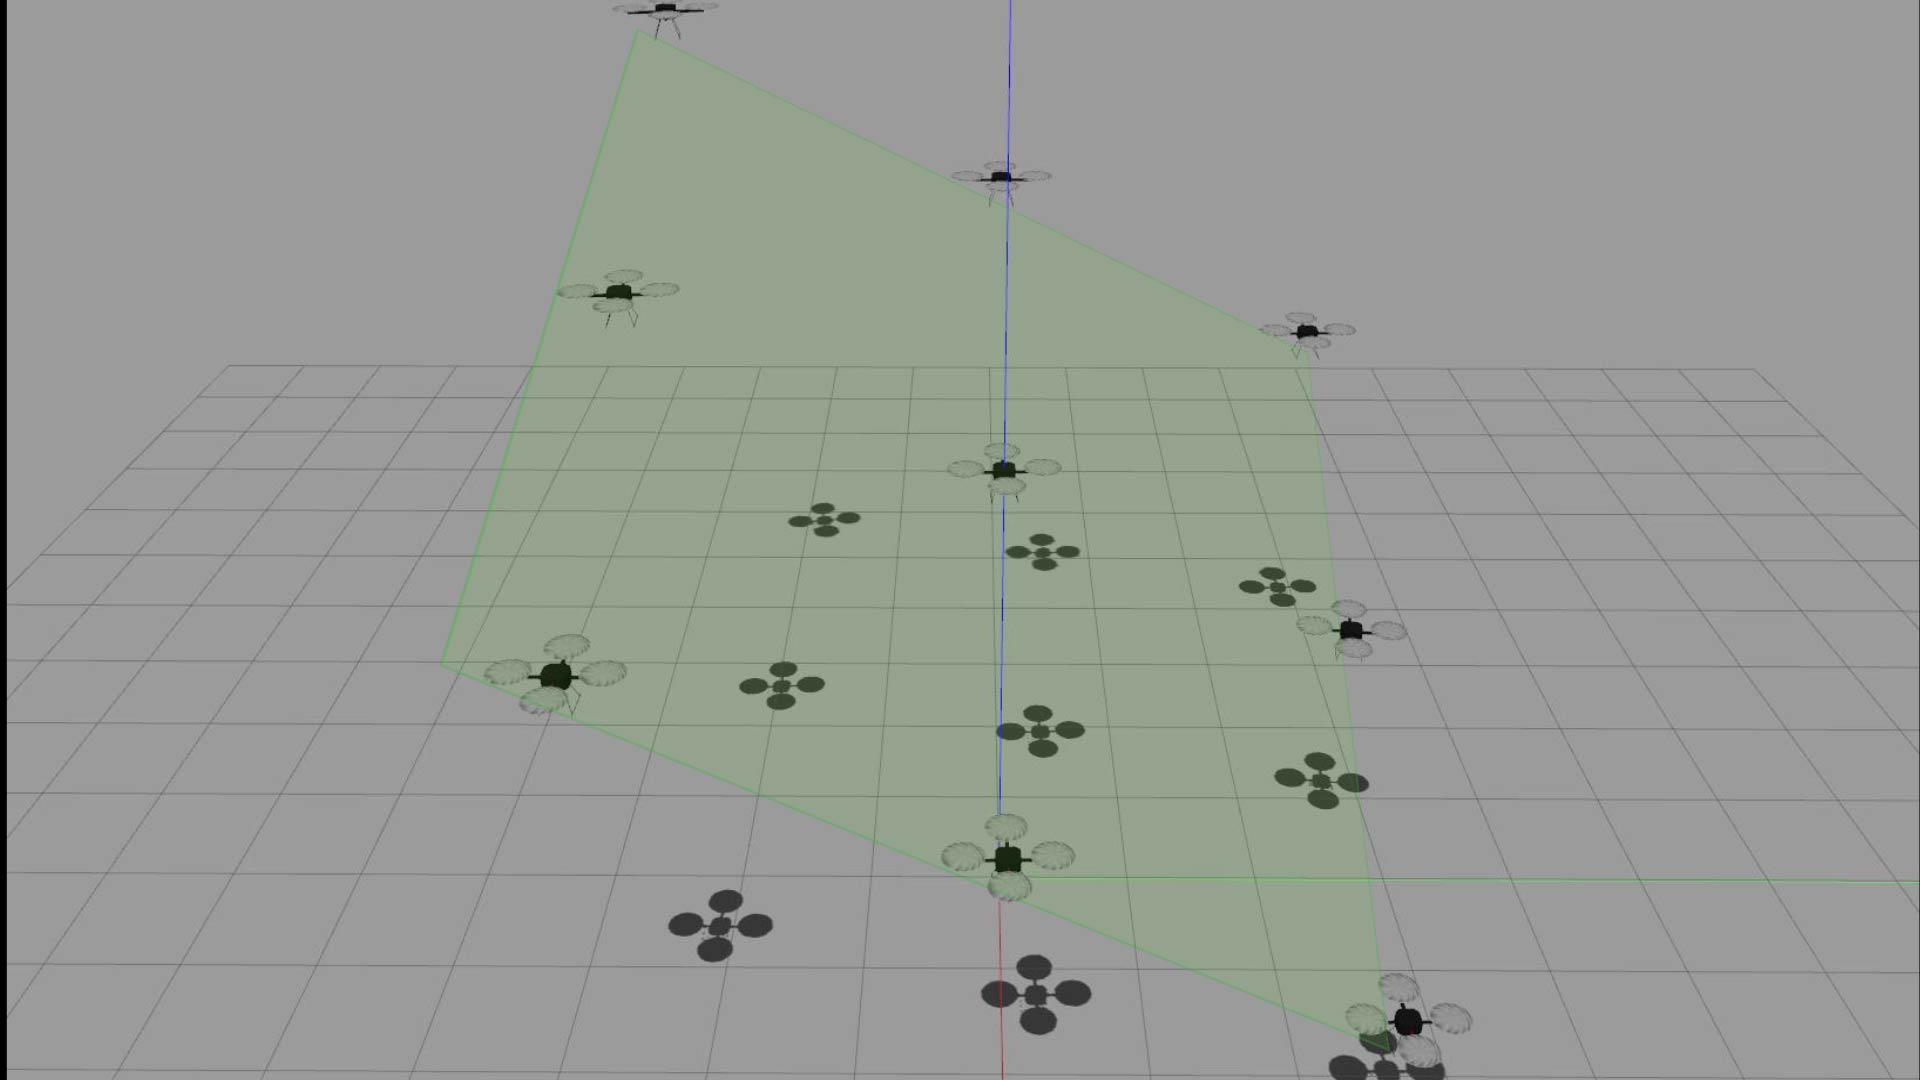
\includegraphics[width=0.33\textwidth]{figs/shapeform_9}
    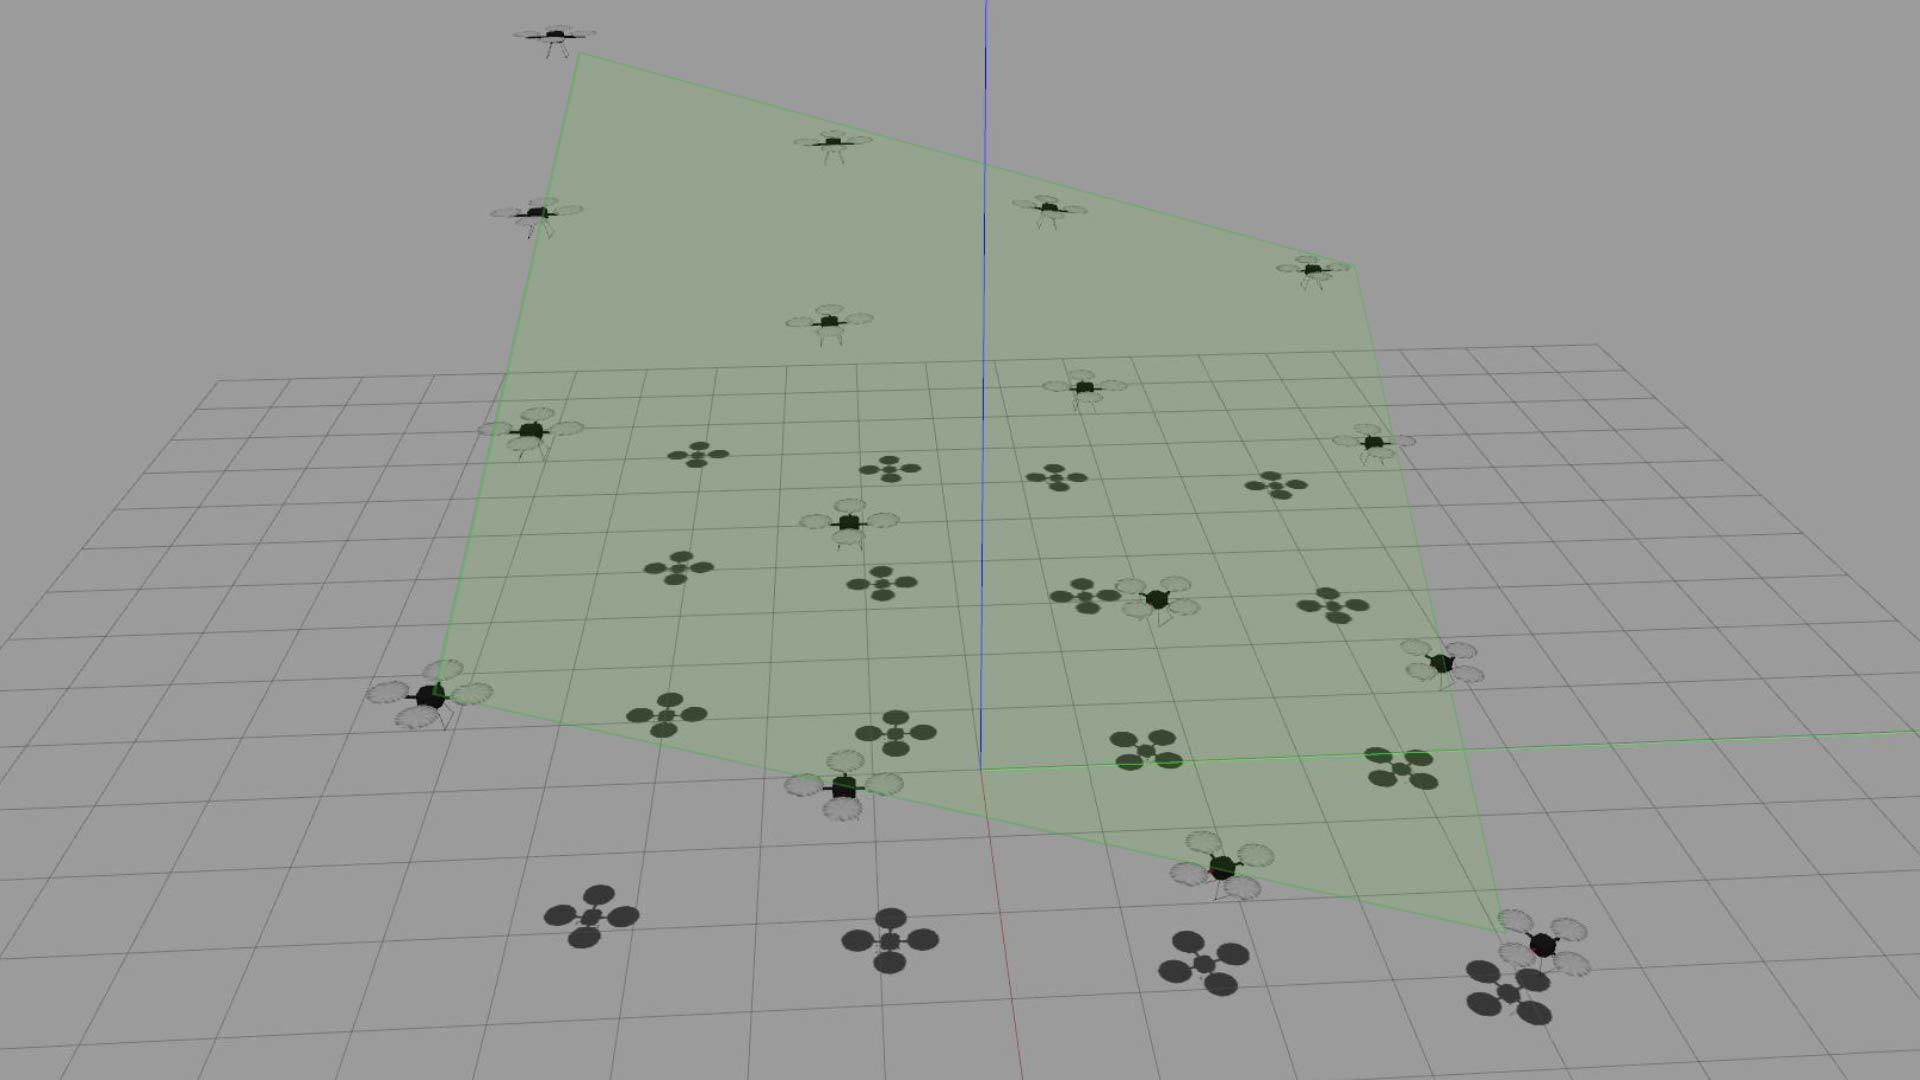
\includegraphics[width=0.33\textwidth]{figs/shapeform_16}
    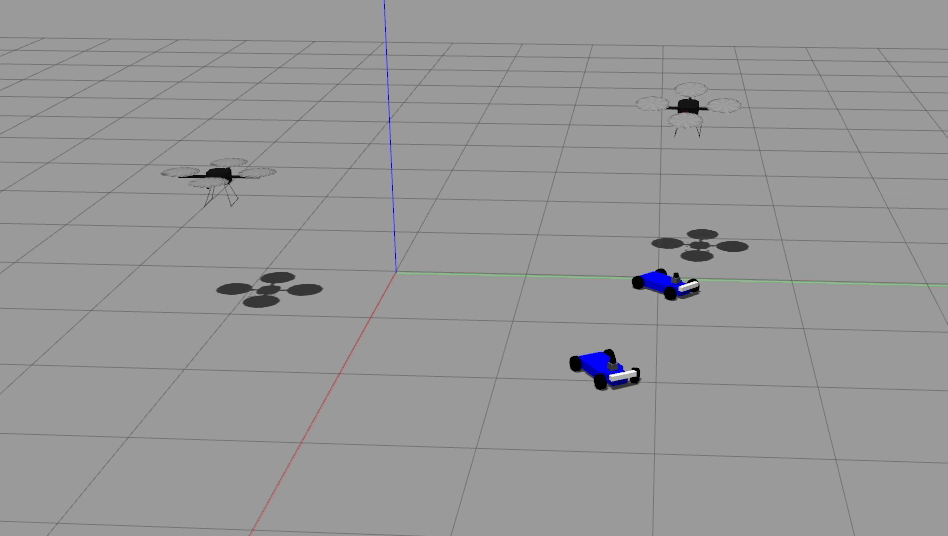
\includegraphics[width=0.33\textwidth]{figs/taskapp_2_2.png}
  \caption{\small CyPhyHouse\ simulator running different scenarios with the same Koord application. \emph{Left} shows simulation of 9 drones running $\Shapeform$ application, \emph{Middle} shows the $\Shapeform$ application on 16 drones. Different scenarios are specified by changing the configuration file.\emph{Right} shows a simulation of $\Task$ on heteterogenous robots. \vspace{-5mm} }
  \label{fig:simexp}
\end{figure*}

\paragraph*{Simulating Koord and communication}
To faithfully simulate the communication, the simulator spawns a process for each robot which encompasses all middleware threads.
The communication handling threads in these processes can then send messages to each other through broadcasts within the local network. To simulate robots on a single machine, the simulator supports specifying distinct network ports for robots in the configuration file. Since the communication is through actual network interfaces, my work can be extended to simulate different network conditions with existing tools in the future.

\paragraph*{Physical Models and Simulated World}
The simulated physical world is developed based on \Gazebo~\cite{gazebo}
and a simulated positioning system is used to relay positions of simulated devices from \Gazebo to the CyPhyHouse middleware.

So far, the implementation includes two \Gazebo robot models from the \Gazebo and ROS community,
the car from the MIT RACECAR project~\cite{MIT_RACECAR} and the quadcopter from the hector quadrotor project~\cite{hector_quadrotor}.
Further, the simulator includes a simplified version of position controller by modifying the provided default model. Users can choose between simplified models for faster simulation or original models for accuracy. In addition to simulation, CyPhyHouse uses Gazebo plugins for visualization. Users may either use these to plot the movements or traces of the robots for real-time monitoring during experiments or visualize and analyze execution traces with Gazebo after experiments.


%This quadratic message complexity arises from both the size of each message for shared memory and the required number of messages
%being linear in the number of robots.
